\section{\name Architecture Overview}
\label{sec:overview}
\name builds on Spark SQL \cite{sparksql} and is optimized specially
for large scale spatial analytics over multi-dimensional spatial data
sets. Because it is based on and extends Spark SQL, it inherits and
extends the SQL query language and the DataFrame API introduced in
Spark SQL, so that users can easily specify different spatial queries
and analytics to interact with the underlying spatial data. A major
challenge in this process is to extend both SQL and the DataFrame
interfaces to support a rich class of spatial operators {\em
  natively inside the \name kernel}.

Figure \ref{fig:architecture} shows the overall architecture of \name.
\name follows a similar architecture as that in Spark SQL, but
introduces new features and components across all stacks. In
particular, new modules that are different from Spark SQL are
highlighted by boxes with orange color in Figure
\ref{fig:architecture}. Similar to Spark SQL, \name allows a user to
interact with the system through command line (CLI), JDBC, and
scala/python programs. The system can connect to a wide variety of
data sources, including those from HDFS (Hadoop Distributed File
System), relational database, Hive, and native RDDs (resilient
distributed datasets).

An important design choice in \name is to stay outside the core spark
engine and only introduce changes to the kernel of Spark SQL. This
choice has made a few implementations more challenging, e.g., adding
the support for spatial operators in query interface and the support
for spatial indexing inside the kernel, but it allows easy migration
of \name into new version of Spark should it be released in the
future.
%\footnote{In fact, we started the design and implementation with
%Spark 1.3 and migrated it to Spark 1.5 when it was released in late 2015.}

%and Users submit their queries or analytical jobs through the {\em
%  programming interface} that supports both SQL

\begin{figure}[t!]
	\centering
	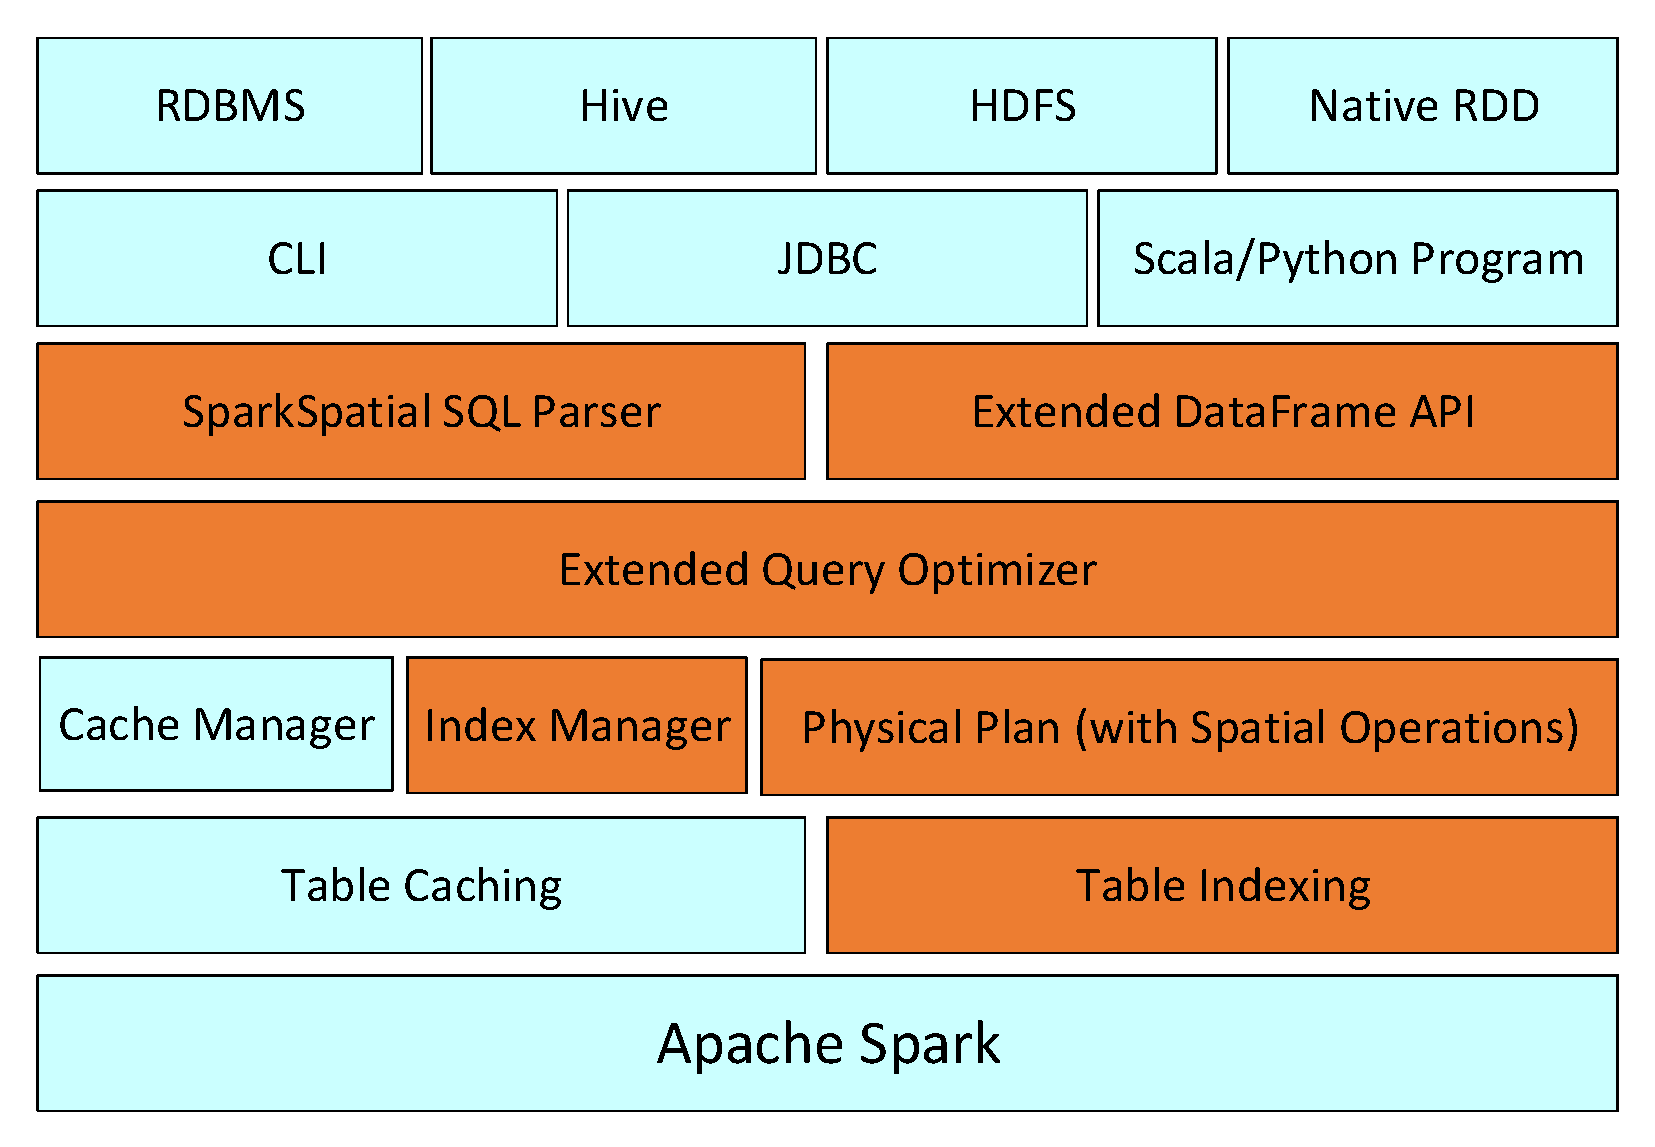
\includegraphics[width = 3.2in]{figs/architecture}
	\vspace{-4mm}
	\caption{\name architecture.}
	\label{fig:architecture}
	\vspace{-4mm}
\end{figure}

\Paragraph{Programming interface.} \name adds spatial
keywords and grammar (e.g. \texttt{POINT}, \texttt{RANGE},
\texttt{KNN}, \texttt{KNN JOIN}, \texttt{DISTANCE JOIN}) in Spark
SQL's query parser, so that user can express spatial queries and
spatial analytical logic in an SQL-like expression. We also extend the
DataFrame API in Spark SQL with similar set of spatial operations,
providing an alternative programming interface for the end user. The
support of spatial operations in the DataFrame API also allows \name
to interchange and interact with other Spark systems easily, such as
SparkML, GraphX, and Spark Streaming. Lastly, we introduce indexing
management to \name's programming interface, in a way that's similar
to that in traditional RDBMS. We will describe the \name's query
interface in details in Section \ref{sec:parser}, and in Appendix
\ref{sec:fullquery}.

\Paragraph{Indexing.} Spatial queries are expensive to process,
especially for data in multi-dimensional space and complex operators
like spatial joins and $\knn$. To achieve efficient and scalable query
performance, \name introduces the concept of {\em indexing} into its
kernel. In particular, \name implements the classic R-tree index
\cite{rtree,DBLP:conf/sigmod/BeckmannKSS90} over the RDD structures in
Spark. \name adopts a two-level indexing strategy: \emph{local} and
\emph{global} indexing. The global index collects statistics from each
RDD partition and helps the system prune irrelevant partitions. Inside
each RDD partition, local indexes are built to accelerate local query
processing, so that linear scan over the entire partition can be
avoided. In \name, user can build and drop indexes anytime on
any table through simple programming interface. Through a construction
called {\em IndexedRDD} which extends the standard RDD structure in
Spark, indexes over RDDs can also be made persistent to disk, and
loaded back, together with associated RDDs, in memory easily. We will
describe the \name's indexing support in Section \ref{sec:index}.

\Paragraph{Spatial operations.} \name supports a number of popular
spatial operations over point and rectangular objects. These spatial
operations are implemented based on the native Spark RDD API. Multiple
access and evaluation paths are provided for each operation, so that
the end users and the \name's query optimizer have the freedom and
opportunities to choose the most appropriate method for a spatial
query or analytical job. Section \ref{sec:query} discusses how various
spatial operations are supported in \name.

\Paragraph{Optimization.} \name extends the logical optimization in
Spark SQL and also introduces a cost-based optimization (CBO) module
that tailors towards optimizing spatial queries. The CBO module
leverages the indexing support in \name, and is able to optimize
complex spatial queries automatically to make the best use of existing
indexes and statistics for the underlying data. Query optimization for
\name is presented in Section \ref{sec:opt}.

\begin{figure}[t!]
  \hspace*{-8mm}
	\centering
	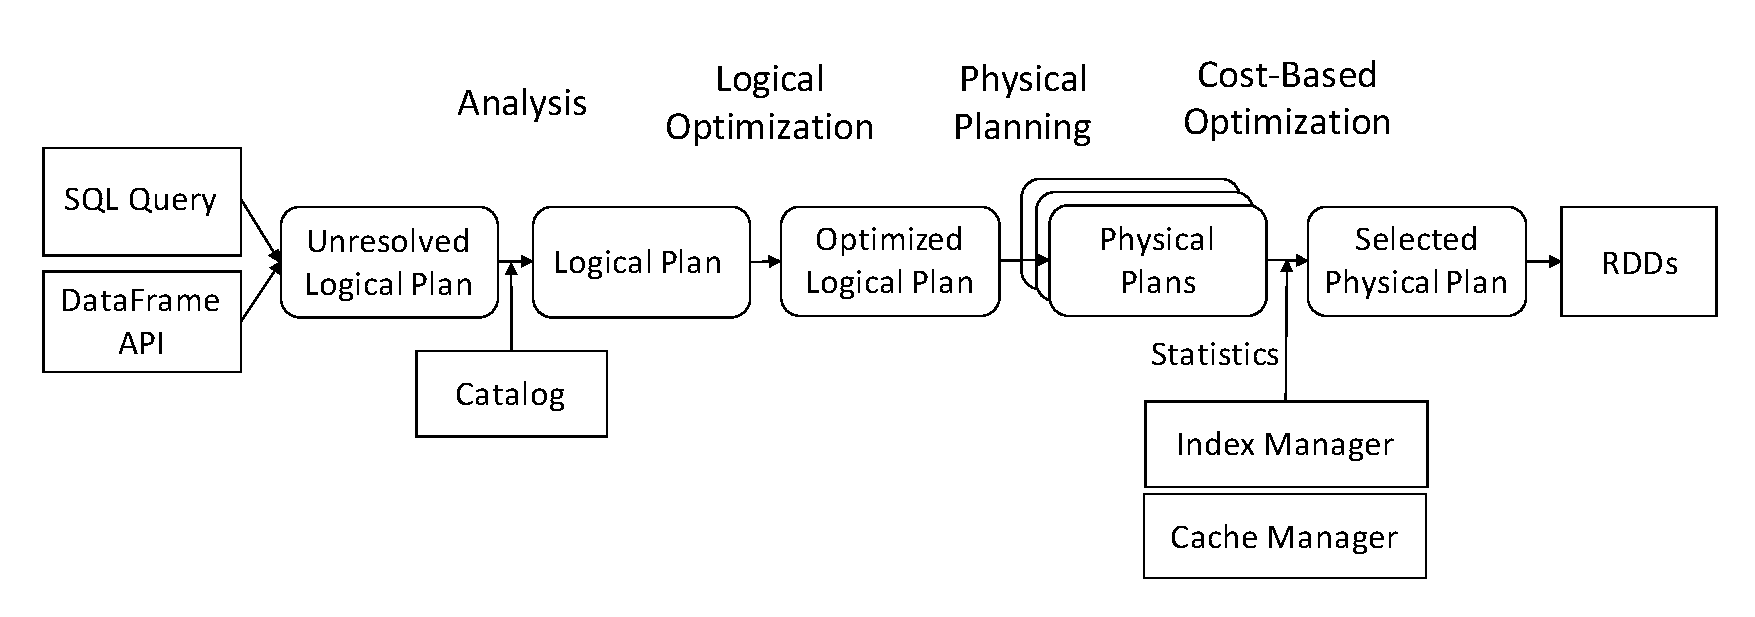
\includegraphics[width = 3.8in]{figs/pipeline}
	\vspace{-8mm}
	\caption{Query processing pipeline in \name.}
	\label{fig:pipeline}
	\vspace{-4mm}
\end{figure}

\Paragraph{Workflow in \name.} Figure \ref{fig:pipeline} shows the
query processing pipeline of \name. \name begins with a relation to be
processed, either from an abstract syntax tree (AST) returned by the
SQL parser or a DataFrame object constructed using the DataFrame
API. In both cases, the relation may contain unresolved attribute
references or relations. An attribute is called {\em unresolved if we
  do not know its type or have not matched it to an input
  table}. \name resolves these attributes with catalyst rules and a
\texttt{Catalog} object that tracks tables in all data sources to
build logical plans. Then, the logical optimizer applies standard
rule-based optimization, such as constant folding, predicate pushdown,
projection pruning, and spatial-specific optimizations such as
distance pruning, to the logical plan. In the physical planing phase,
\name takes a logical plan as input and generates one or more physical
plans based on the spatial operations supported by \name, as well as
using physical operators implemented within Spark's execution
engine. It then applies a cost-based optimizer based on {\em
  statistics collected in both Cache Manager and Index Manager} to
select the most efficient plan.  The physical planner also performs
rule-based physical optimization, such as pipelining projections or
combining filters into one Spark \texttt{map} operation. In addition,
it can push operations from the logical plan into data sources that
support predicate or projection pushdown.

\name supports analytical jobs on various data sources such as CVS,
JSON and JDBC. Figure \ref{fig:storage} shows how data are represented
in \name.  Generally speaking, each data source will be transformed to
an RDD of records (i.e., \texttt{RDD[Row]}) for further
evaluation. \name allows users to materialize (often referred as
``cache'') hot data in memory using columnar storage, which can reduce
memory footprint by an order of magnitude because it relies on Spark
SQL to apply columnar compression schemes such as dictionary encoding
and run-length encoding. Besides, user can build various indexes
(e.g. hash maps, tree maps, R-trees) over different datasets to
accelerate interactive query processing.

%%% Local Variables:
%%% mode: latex
%%% TeX-master: "paper"
%%% End:
